\documentclass[border = 2mm]{standalone}
\usepackage[utf8]{inputenc}
\usepackage{tikz}
\usetikzlibrary{arrows.meta, calc}

% Assembly plan of the shelter (Stevenson screen), dimensions in cm.
% Four louvered vent grilles of 23 x 23 cm are screwed on four corner
% battens; a drilled bottom board below, a double roof above, which is
% also the lid. The sealed box of the electronics sits at the bottom,
% the air sensors hang under the roof, the solar panel lies on it.

\tikzset{
    wood/.style={draw, thick, fill=orange!25},
    grille/.style={draw, thick, fill=white},
    louver/.style={gray, thick},
    hidden/.style={draw, dashed, gray},
    metal/.style={draw, thick, fill=gray!40},
    panel/.style={draw, thick, fill=blue!40},
    cable/.style={thick, blue!70!black},
    dim/.style={{Latex[length=1.5mm]}-{Latex[length=1.5mm]}, thin},
    dimtext/.style={font=\sffamily\scriptsize, fill=white, inner sep=1pt},
    note/.style={font=\sffamily\scriptsize, align=left},
    title/.style={font=\sffamily\bfseries\small},
}

% A grille seen from the front: its frame and its slanted louvers
\newcommand{\grillefront}[4]{% x, y, width, height
    \draw[grille] (#1,#2) rectangle ++(#3,#4);
    \foreach \k in {1,...,12} {
        \draw[louver] ($(#1,#2)+(0.8,{\k*#4/13})$) -- ++({#3-1.6},0);
    }
}

\begin{document}
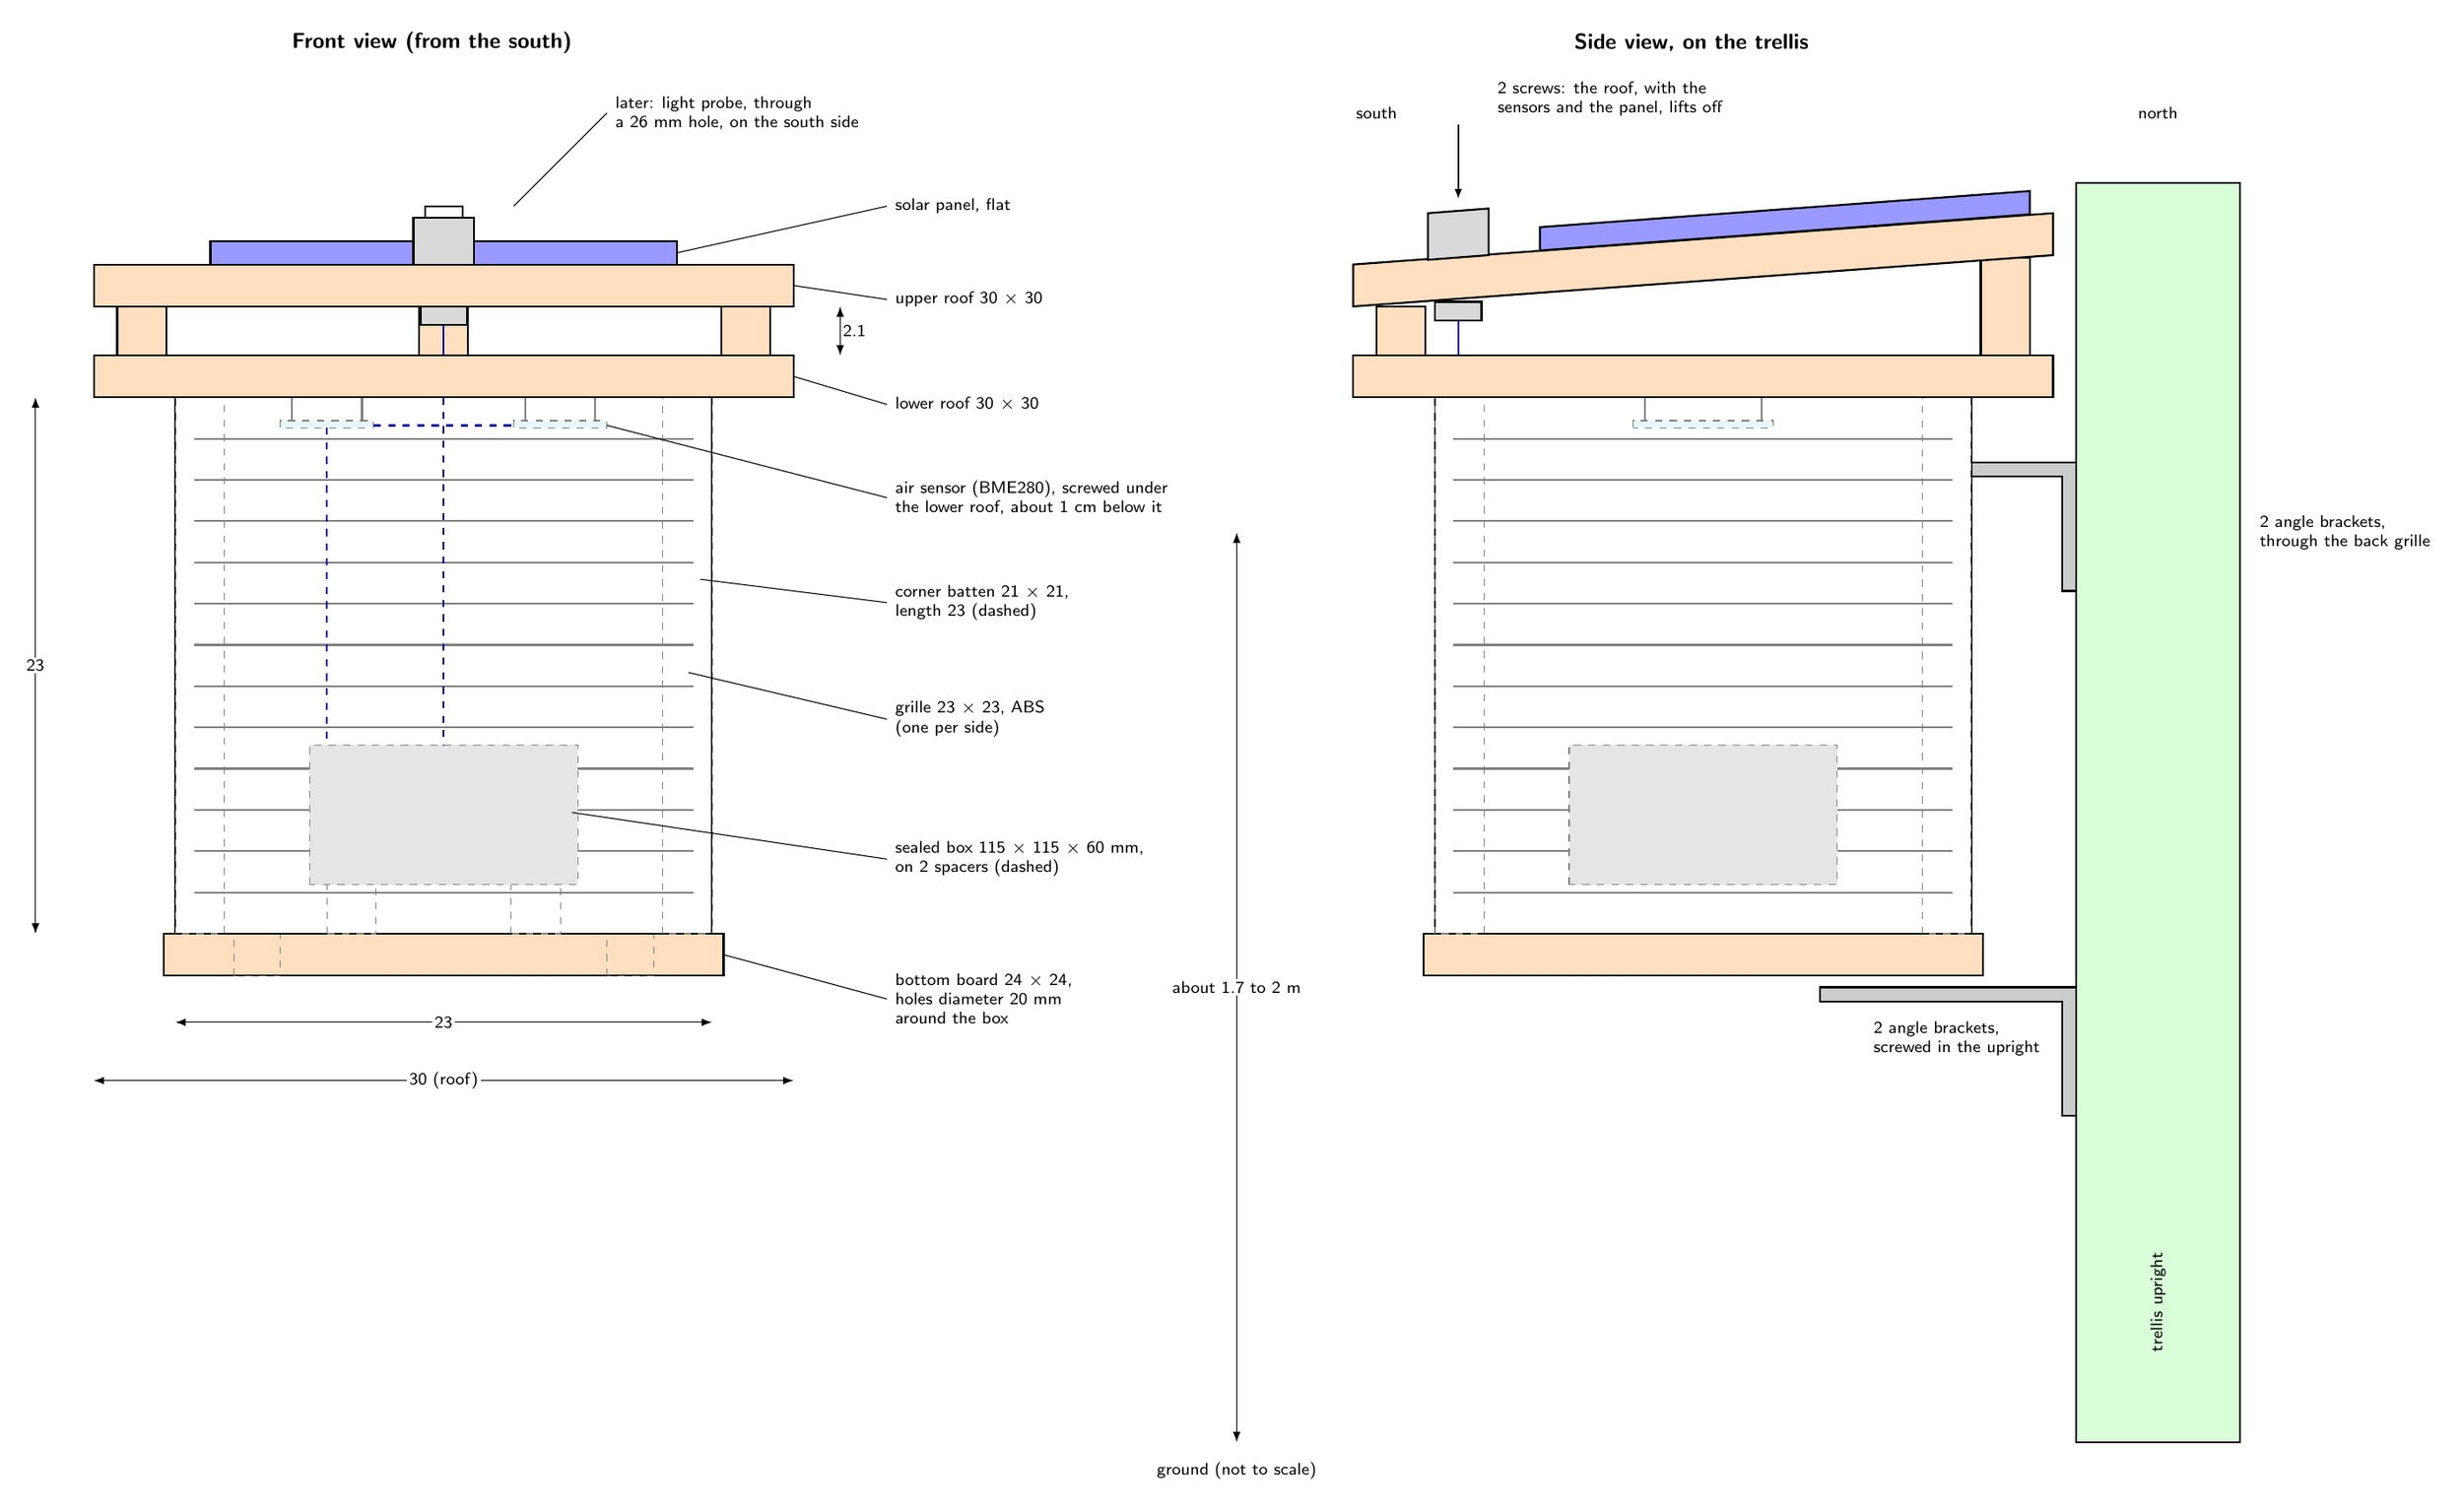
\begin{tikzpicture}[scale=0.34]

% ================================================================ front view
% Seen from the south: the front of the shelter faces the sun at noon
\node[title] at (11.5,40) {Front view (from the south)};

% bottom board 24 x 24 x 1.8, drilled
\draw[wood] (0,0) rectangle (24,1.8);
\foreach \x in {4,20} { \draw[hidden] (\x-1,0) rectangle (\x+1,1.8); }

% front grille 23 x 23, on the corner battens (dashed, behind it)
\grillefront{0.5}{1.8}{23}{23}
\draw[hidden] (0.5,1.8) rectangle (2.6,24.8);
\draw[hidden] (21.4,1.8) rectangle (23.5,24.8);

% the sealed box of the electronics, on two spacers, at the bottom
\draw[hidden] (7,1.8) rectangle (9.1,3.9);
\draw[hidden] (14.9,1.8) rectangle (17,3.9);
\draw[hidden, fill=gray!20] (6.25,3.9) rectangle (17.75,9.9);

% the two air sensors, screwed under the lower roof on 1 cm nylon
% standoffs: they touch no wall, and the air goes all around them
\foreach \x in {5.5,8.5,15.5,18.5} { \draw[thick, gray] (\x,23.8) -- (\x,24.8); }
\draw[hidden, fill=cyan!10] (5,23.5) rectangle (9,23.8);
\draw[hidden, fill=cyan!10] (15,23.5) rectangle (19,23.8);
\draw[cable, dashed] (9,23.6) -- (15,23.6);
\draw[cable, dashed] (7,23.5) -- (7,9.9);

% lower roof 30 x 30, spacers, upper roof 30 x 30
\draw[wood] (-3,24.8) rectangle (27,26.6);
\draw[wood] (-2,26.6) rectangle (0.1,28.7);
\draw[wood] (10.95,26.6) rectangle (13.05,28.7);
\draw[wood] (23.9,26.6) rectangle (26,28.7);
\draw[wood] (-3,28.7) rectangle (27,30.5);

% on the roof: the solar panel, lying flat, and the light probe, screwed
% through the upper board; its cable goes down through a small hole of
% the lower board, sheltered by the upper one
\draw[panel] (2,30.5) rectangle (22,31.5);
\draw[thick, fill=gray!30] (10.7,30.5) rectangle (13.3,32.5);
\draw[thick, fill=white] (11.2,32.5) rectangle (12.8,33);
\draw[thick, fill=gray!30] (11,27.9) rectangle (13,28.7);
\draw[cable] (12,27.9) -- (12,26.6);
\draw[cable, dashed] (12,24.8) -- (12,9.9);

% dimensions
\draw[dim] (0.5,-2) -- (23.5,-2) node[dimtext, midway] {23};
\draw[dim] (-3,-4.5) -- (27,-4.5) node[dimtext, midway] {30 (roof)};
\draw[dim] (-5.5,1.8) -- (-5.5,24.8) node[dimtext, midway] {23};
\draw[dim] (29,26.6) -- (29,28.7) node[dimtext, midway, right] {2.1};

% labels
\draw[thin] (24,0.9) -- (31,-1) node[note, anchor=west] {bottom board 24 $\times$ 24,\\holes diameter 20 mm\\around the box};
\draw[thin] (17.5,7) -- (31,5) node[note, anchor=west] {sealed box 115 $\times$ 115 $\times$ 60 mm,\\on 2 spacers (dashed)};
\draw[thin] (22.5,13) -- (31,11) node[note, anchor=west] {grille 23 $\times$ 23, ABS\\(one per side)};
\draw[thin] (23,17) -- (31,16) node[note, anchor=west] {corner batten 21 $\times$ 21,\\length 23 (dashed)};
\draw[thin] (19,23.6) -- (31,20.5) node[note, anchor=west] {air sensor (BME280), screwed under\\the lower roof, about 1 cm below it};
\draw[thin] (27,25.7) -- (31,24.5) node[note, anchor=west] {lower roof 30 $\times$ 30};
\draw[thin] (27,29.6) -- (31,29) node[note, anchor=west] {upper roof 30 $\times$ 30};
\draw[thin] (22,31) -- (31,33) node[note, anchor=west] {solar panel, flat};
\draw[thin] (15,33) -- (19,37) node[note, anchor=west] {later: light probe, through\\a 26 mm hole, on the south side};

% ================================================================ side view
\begin{scope}[shift={(54,0)}]
\node[title] at (11.5,40) {Side view, on the trellis};
\node[note] at (-2,37) {south};
\node[note] at (31.5,37) {north};

% upright of the garden trellis, behind the shelter
\draw[wood, fill=green!15] (28,-20) rectangle (35,34);
\node[note, rotate=90] at (31.5,-14) {trellis upright};

% angle brackets under the bottom board
\draw[metal] (17,-0.5) -- (28,-0.5) -- (28,-6) -- (27.4,-6) -- (27.4,-1.1) -- (17,-1.1) -- cycle;
\node[note, anchor=north east] at (26.8,-1.6) {2 angle brackets,\\screwed in the upright};

% 2 more brackets at the top, screwed through the back grille into the
% back corner battens: the lid stays free
\draw[metal] (23.5,22) -- (28,22) -- (28,16.5) -- (27.4,16.5) -- (27.4,21.4) -- (23.5,21.4) -- cycle;
\node[note, anchor=west] at (35.5,19) {2 angle brackets,\\through the back grille};

% bottom board, side grille, battens, box, sensors
\draw[wood] (0,0) rectangle (24,1.8);
\grillefront{0.5}{1.8}{23}{23}
\draw[hidden] (0.5,1.8) rectangle (2.6,24.8);
\draw[hidden] (21.4,1.8) rectangle (23.5,24.8);
\draw[hidden, fill=gray!20] (6.25,3.9) rectangle (17.75,9.9);
\foreach \x in {9.5,14.5} { \draw[thick, gray] (\x,23.8) -- (\x,24.8); }
\draw[hidden, fill=cyan!10] (9,23.5) rectangle (15,23.8);

% lower roof, flat; spacers: 1 batten at the front, 2 stacked at the back
\draw[wood] (-3,24.8) rectangle (27,26.6);
\draw[wood] (-2,26.6) rectangle (0.1,28.7);
\draw[wood] (23.9,26.6) rectangle (26,30.8);
% upper roof, sloped to the south: the rain runs off away from the trellis,
% and the panel faces the sun a little better
\draw[wood] (-3,28.7) -- (27,30.9) -- (27,32.7) -- (-3,30.5) -- cycle;
% panel lying on it, light probe on the south strip
\draw[panel] (5,31.1) -- (26,32.65) -- (26,33.65) -- (5,32.1) -- cycle;
\draw[thick, fill=gray!30] (0.2,30.7) -- (2.8,30.9) -- (2.8,32.9) -- (0.2,32.7) -- cycle;
\draw[thick, fill=gray!30] (0.5,28.1) rectangle (2.5,28.9);
\draw[cable] (1.5,28.1) -- (1.5,26.6);

% the roof is the lid: 2 wood screws into 2 opposite corner battens
\draw[thick, -{Latex[length=1.5mm]}] (1.5,36.5) -- (1.5,33.3);
\node[note, anchor=south] at (8,36.5) {2 screws: the roof, with the\\sensors and the panel, lifts off};

% height
\draw[dim] (-8,-20) -- (-8,19) node[dimtext, midway] {about 1.7 to 2 m};
\node[note, anchor=north] at (-8,-20.5) {ground (not to scale)};
\end{scope}

\end{tikzpicture}
\end{document}
